\documentclass[fleqn, a4paper, 12pt]{article}
\usepackage{amsmath, amssymb, amsthm}
\usepackage{gensymb}
\usepackage{commath}
\usepackage{xcolor}
\usepackage{cancel}
\usepackage{siunitx}
\usepackage{tikz, pgfplots}
	\usetikzlibrary{calc, hobby, patterns, intersections}
\usepackage{graphicx}
\usepackage{hyperref}
\usepackage{datetime}
\usepackage{ulem}
\usepackage{xfrac}
\usepackage{asymptote}
\usepackage{enumerate}
\setcounter{secnumdepth}{4}
\newcommand\numberthis{\addtocounter{equation}{1}\tag{\theequation}}

\newcommand{\AxisRotator}[1][rotate=0]{%
	\tikz [x=0.25cm,y=0.60cm,line width=.2ex,-stealth,#1] \draw (0,0) arc (-150:150:1 and 1);%
}

\theoremstyle{definition}
\newtheorem{example}{Example}
\newtheorem{definition}{Definition}

\theoremstyle{theorem}
\newtheorem{theorem}{Theorem}

\newenvironment{solution}
{\begin{proof}[Solution]\let\qed\relax}
	{\end{proof}}

\newcommand{\curl}{\mathrm{curl\,}}

%\renewcommand{\int_{min}^{max}}{\int\displaylimits_{min}^{max}}

%opening
\title{Lecture 21}
\author{Aakash Jog}
\date{\formatdate{8}{1}{2015}}

\begin{document}

\maketitle
%\setlength{\mathindent}{0pt}

\tableofcontents

\newpage
\section{Forced Oscillations}

\begin{example}
	Find\\
	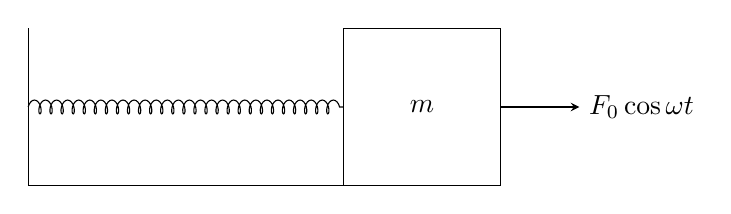
\begin{tikzpicture}
		\def\l{4};
		\def\x{0};
		\def\segmentlength{4};
		\def\F{1};
		
		\draw (0,2) -- (0,0) -- ({\l + \x},0);
		
		\draw [decorate, decoration = {coil, segment length = {(\l + \x)/(\l)*\segmentlength}}](0,1) -- ({\l + \x},1);
		
		\draw ({\l + \x},2) rectangle  node {$m$} ({\l + \x + 2}, 0);

		\draw [-stealth] ({\l + \x + 2}, 1) -- ++(0:\F) node [right] {$F_0 \cos \omega t$};
	\end{tikzpicture}
\end{example}

\begin{solution}
	\hspace{1cm}\\
	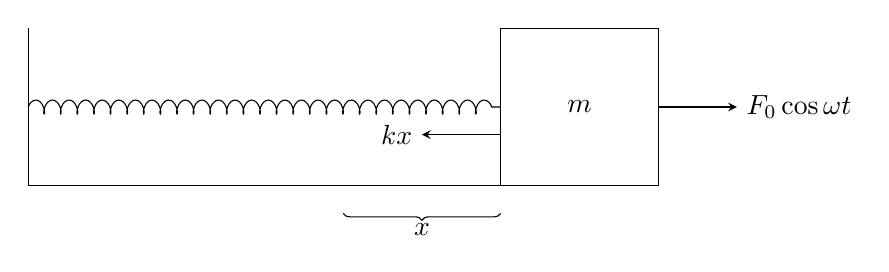
\begin{tikzpicture}
		\def\l{4};
		\def\x{2};
		\def\segmentlength{4};
		\def\F{1};
		
		\draw (0,2) -- (0,0) -- ({\l + \x},0);
		
		\draw [decorate, decoration = {coil, segment length = {(\l + \x)/(\l)*\segmentlength}}](0,1) -- ({\l + \x},1);
		
		\draw ({\l + \x},2) rectangle  node {$m$} ({\l + \x + 2}, 0);
		
		\draw [decorate, decoration = {mirror, brace}, yshift = -10] (\l,0) -- ({\l + \x},0) node [midway, below] {$x$};
		
		\draw [-stealth] ({\l + \x + 2}, 1) -- ++(0:\F) node [right] {$F_0 \cos \omega t$};
		
		\draw [-stealth, yshift = -10] ({\l + \x}, 1) -- ++(180:\F) node [left] {$kx$};
	\end{tikzpicture}
	\begin{align*}
		m \ddot{x} + \dfrac{k}{m} x &= \dfrac{F_0}{m} \cos \omega t\\
		\therefore \ddot{x} + \dfrac{k}{m} x &= \dfrac{F_0}{m} \cos \omega t
	\end{align*}
	Therefore, solving
	\begin{align*}
		x &= A \cos \omega_0 t + B \sin \omega_0 t + \dfrac{F_0}{k - m \omega^2} \cos \omega t\\
		\therefore \dot{x} &= \omega_0 (-A \sin \omega_0 t + B \cos \omega_0 t) - \dfrac{F_0}{k - m \omega^2} \omega \sin \omega t
	\end{align*}
	Substituting initial conditions,
	\begin{align*}
		x &= \dfrac{\dfrac{F_0}{m}}{\dfrac{k}{m} - \omega^2} (-\cos \omega_0 t + \cos \omega t)\\
		\intertext{Let $\dfrac{F_0}{m} = f_0$}
		\therefore x &= -\dfrac{2 f_0}{{\omega_0}^2 - \omega^2} \sin \left( \dfrac{\omega t - \omega_0 t}{2} \right) \sin \left( \dfrac{\omega t + \omega_0 t}{2} \right)\\
		\intertext{$\omega - \omega_0 = \Delta \omega$ and $\omega + \omega_0 \approx 2 \omega_0$}
		\therefore x &\approx \dfrac{2 f_0}{\Delta \omega \cdot 2 \omega_0} \sin \left( \dfrac{\Delta \omega}{2} t \right) \cdot \sin (\omega_0 t)
	\end{align*}
\end{solution}

\end{document}